\begin{center}
	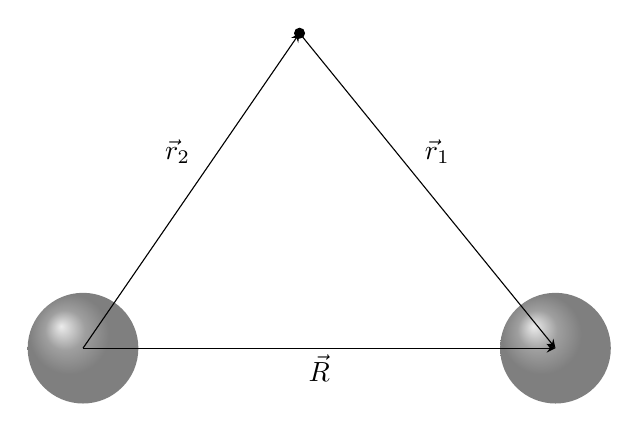
\begin{tikzpicture}		
		\shade[ball color = black,
		opacity = 0.5
		] (-3,0,0) circle (20pt);
		
		
		\shade[ball color = black,
		opacity = 0.5
		] (3,0,0) circle (20pt);
		
		
		\fill[black] (-0.25, 4, 0) circle (2pt) ;
		
		\draw[-{stealth[scale=2]}] (-3, 0, 0) -- (3, 0, 0);
		
		\draw[-{stealth[scale=2]}] (-3, 0, 0) -- (-0.25, 4, 0);
		
		\draw[{stealth[scale=2]}-] (3, 0, 0) -- (-0.25, 4, 0);
		
		\draw (0, -0.25, 0) node {$\vec R$};
		
		\draw (1.5, 2.5, 0) node {$\vec r_1$};
		
		\draw (-1.8, 2.5, 0) node {$\vec r_2$};
		
	\end{tikzpicture}
\end{center}
